\documentclass[template.tex]{subfiles}
\begin{document}

\xchapter{Resultados obtidos}{}

Nessa seção são descritos e discutidos os experimentos realizados e os resultados obtidos desses experimentos. O objetivo é não só comparar qual cenário obtém melhor \textit{acuracia} ou TPR e TNR, mas também discutir em quais contextos os classificadores produzem melhores ou piores resultados.

%\section{Datasets}
\todo[inline]{Pelo que vi nos comentários da seção de metodologia essa seção deve sumir daqui e subir para para metodologia, certo?}
\todo[inline]{Isso mesmo, vai para metodologia, mas cuidado com duplicações de conteúdo lá}
\todo[inline]{matheus: Já tinha escrito bem na metodologia então somente removi. Essa subseção se foi}

%\section{Resultados experimentais}

Nós focamos em comparar os métodos de seleção de características e de inferência, variando as configurações em diferentes etapas do processo de mineração de opinião, comparando acurácia, TPR e TNR. Nós avaliamos a influência dos algoritmos de seleção de características, os sistemas de inferência fuzzy em si, o uso de pesos na regras, a quantidade usada de conjuntos fuzzy, a eficiência das regras entre domínios e usadas em outro,características mais selecionadas entre as bases utilizadas. 

\todo[inline]{usa folds ao inves de dobras, já troquei no parágrafo abaixo e refiz redação também}
\todo[inline]{matheus: ok}

\todo[inline]{matheus: esse paragrafo ja tem na metodologia. Daí eu eliminei e juntei com o paragrafo do inicio do capitulo e eliminei essa seção também. O texto eliminado está comentádo no latex.}
%Para cada base de dados, o processo de mineração de opinião é idêntico para as etapas de pré-processamento, transformação e extração de características. Aplicando validação cruzada de 10 folds, as 9 partes da base são utilizadas para treinamento são utilizadas para seleção de características, na modelagem dos conjuntos fuzzy e na construção da base de regras fuzzy. A parte restante é utilizada somente para teste, realizando a seleção da mesmas características escolhidas durante o treino e fornecendo os valores destas para o sistema fuzzy realizar a classificação. O mesmo processo é repetido para cada fold e os resultados, para todas as medidas usadas, são a média dos valores obtidos em cada fold de teste. 

\todo[inline]{falta mais discussão nas seções seguintes, apresente mais informações sobre o que ocorreu, e discuta os resultados a luz do comportamento do sistema}

Nossos resultados são fruto de uma uma extensa quantidade de combinações nas duas bases de dados, filmes e Amazon, entre os algoritmos de seleção de características, os tipos sistemas de inferência fuzzy (utilizando pesos na regras ou não) e a quantidade usada de conjuntos fuzzy para modelar as variáveis de entrada. É importante observar que o algoritmo c4.5 é mostrado com duas variações: altura 1 e 2. Deixando o algoritmo construir livremente a árvore do decisão para a seleção de características, em dois cenários diferentes, nós escolhemos utilizar as características que estavam nos nós das árvores até altura 1 e 2. Isso resultou na mudança da quantidade de características selecionadas nos dois cenários. Fizemos isso para analisar também em quanto a altura da árvore de decisão do c4.5 influenciaria nos resultados. Vale notar que fizemos até altura 3, mas as características selecionadas eram as mesmas para altura 2. 
As tabelas \ref{table:movies_3f} e \ref{table:movies_2f} mostram os resultados na base de filmes e as tabelas \ref{table:amazon_3f} e \ref{table:amazon_2f} na base mista da Amazon. Primeiramente vamos discutir os cenários para o uso de 3 conjuntos fuzzy e depois para o uso de somente 2.

\begin{table}[H]
\begin{tabular}{ @{} c*{11}c @{} }
	\rot{CFS} & \rot{C4.5 - Altura 1} & \rot{C4.5 - Altura 2} & \rot{MRFG} & \rot{MRFG C/ PESOS} & \rot{MRFC} & \rot{MRFC C/ PESOS} & \rot{ACURÁCIA} & \rot{TNR} & \rot{TPR}  \\ \hline
	X &  &  & X &  &  &  & 62.9\% +- 4.25\% & 63.1\% +- 22.46\% & 62.7\% & 22.69\% \\ \hline
	X &  &  &  & X &  &  & 67.1\% +- 3.39\% & 72.6\% +- 8.77\% & 61.6\% & 9.77\% \\ \hline
	X &  &  &  &  & X &  & 52.25\% +- 4.92\% & 40.3\% +- 32.94\% & 64.2\% & 30.55\% \\ \hline
	X &  &  &  &  &  & X & 56.2\% +- 5.16\% & 55.1\% +- 19.21\% & 57.3\% & 14.26\% \\ \hline
	 & X &  & X &  &  &  & 59.2\% +- 1.83\% & 53.8\% +- 34.96\% & 64.6\% & 37.08\% \\ \hline
	 & X &  &  & X &  &  & 70.05\% +- 0.04 & 70.4\% +- 7.11\% & 69.7\% & 9.81\% \\ \hline
	 & X &  &  &  & X &  & 54.4\% +- 1.72\% & 47.1\% +- 42.67\% & 61.7\% & 43.93\% \\ \hline
	 & X &  &  &  &  & X & 69.8\% +- 4.03\% & 69.3\% +- 10.15\% & 70.3\% & 11.73\% \\ \hline
	 &  & X & X &  &  &  & 59.65\% +- 2.42\% & 60.3\% +- 35.78\% & 0.59 & 36.9\% \\ \hline
	 &  & X &  & X &  &  & 70\% +- 3.96\% & 70.3\% +- 7.02\% & 69.7\% & 9.81\% \\ \hline
	 &  & X &  &  & X &  & 54.5\% +- 1.76\% & 55.6\% +- 43.49\% & 53.4\% & 44.5\% \\ \hline
	 &  & X &  &  &  & X & 69.8\% +- 4.03\% & 69.3\% +- 10.15\% & 70.3\% & 11.73\% \\ \hline
\end{tabular}
\caption{Resultados da base de filmes, utilizando 3 conjuntos fuzzy nas variáveis de entrada}
\label{table:movies_3f}
\end{table}
	
\begin{table}[H]
\begin{tabular}{ @{} c*{11}c @{} }
	\rot{CFS} & \rot{C4.5 - Altura 1} & \rot{C4.5 - Altura 2} & \rot{MRFG} & \rot{MRFG C/ PESOS} & \rot{MRFC} & \rot{MRFC C/ PESOS} & \rot{ACURÁCIA} & \rot{TNR} & \rot{TPR} \\ \hline
	X &  &  & X &  &  &  & 67.35\% +- 6.36\% & 57.8\% +- 11.83\% & 76.9\% +- 11.39\% \\ \hline
	X &  &  &  & X &  &  & 68.85\% +- 6.66\% & 62.4\% +- 9.72\% & 75.3\% +- 11.61\% \\ \hline
	X &  &  &  &  & X &  & 64.4\% +- 8.12\% & 51.3\% +- 13.56\% & 77.5\% +- 13.90\% \\ \hline
	X &  &  &  &  &  & X & 67.55\% +- 6.14\% & 58.2\% +- 10.04\% & 76.9\% +- 11.51\% \\ \hline
	 & X &  & X &  &  &  & 60.05\% +- 2.37\% & 44.6\% +- 35.73\% & 75.5\% +- 34.8\% \\ \hline
	 & X &  &  & X &  &  & 70.85\% +- 3.09\% & 76.8\% +- 4.57\% & 64.9\% +- 5.5\% \\ \hline
	 & X &  &  &  & X &  & 54.25\% +- 2.82\% & 34\% +- 43.26\% & 74.5\% +- 38.82\% \\ \hline
	 & X &  &  &  &  & X & 70.55\% +- 3.12\% & 75.2\% +- 5.68\% & 65.9\% +- 6.25\% \\ \hline
	 &  & X & X &  &  &  & 61.75\% +- 4.2\% & 79.4\% +- 29.30\% & 44.1\% +- 31.92\% \\ \hline
	 &  & X &  & X &  &  & 68.85\% +- 3.27\% & 85.4\% +- 8.27\% & 52.3\% +- 12.82\% \\ \hline
	 &  & X &  &  & X &  & 60.4\% +- 5.75\% & 73.7\% +- 35.86\% & 47.1\% +- 34.22\% \\ \hline
	 &  & X &  &  &  & X & 68.15\% +- 2.84\% & 80.4\% +- 8.91\% & 55.9\% +- 12.87\% \\ \hline
\end{tabular}
\caption{Resultados da base da Amazon, utilizando 3 conjuntos fuzzy nas variáveis de entrada}
\label{table:amazon_3f}
\end{table}

\begin{table}[H]
\begin{tabular}{ @{} c*{11}c @{} }
	\rot{CFS} & \rot{C4.5 - Altura 1} & \rot{C4.5 - Altura 2} & \rot{MRFG} & \rot{MRFG C/ PESOS} & \rot{MRFC} & \rot{MRFC C/ PESOS} & \rot{ACURÁCIA} & \rot{TNR} & \rot{TPR}  \\ \hline
	X &  &  & X &  &  &  & 68.60\% +- 7.6\% & 74.9\% +- 9.52\% & 62.3\% +- 13.84\% \\ \hline
	X &  &  &  & X &  &  & 69.05\% +- 7.59\% & 68.4\% +- 24.26\% & 69.7\% +- 13.15\% \\ \hline
	X &  &  &  &  & X &  & 66.75\% +- 7.97\% & 59.7\% +- 17.60\% & 73.8\% +- 7.79\% \\ \hline
	X &  &  &  &  &  & X & 67.5\% +- 6.73\% & 63.8\% +- 22.45\% & 71.2\% +- 12.63\% \\ \hline
	 & X &  & X &  &  &  & 70.55\% +- 3.40\% & 71.4\% +- 5.71\% & 69.7\% +- 6.03\% \\ \hline
	 & X &  &  & X &  &  & 70.9\% +- 3.07\% & 71.2\% +- 4.33\% & 70.6\% +- 3.35\% \\ \hline
	 & X &  &  &  & X &  & 70.55\% +- 3.40\% & 71.4\% +- 5.71\% & 69.7\% +- 6.03\% \\ \hline
	 & X &  &  &  &  & X & 70.9\% +- 3.07\% & 71.2\% +- 4.33\% & 70.6\% +- 3.35\% \\ \hline
	 &  & X & X &  &  &  & 70.55\% +- 3.4\% & 71.2\% +- 5.54\% & 69.9\% +- 6.04\% \\ \hline
	 &  & X &  & X &  &  & 69.65\% +- 4.12\% & 0.67 +- 12.74\% & 72.3\% +- 6.98\% \\ \hline
	 &  & X &  &  & X &  & 70.55\% +- 3.4\% & 71.4\% +- 5.71\% & 69.7\% +- 6.03\% \\ \hline
	 &  & X &  &  &  & X & 70.9\% +- 3.07\% & 71.2\% +- 4.33\% & 70.6\% +- 3.35\% \\ \hline
\end{tabular}
\caption{Resultados da base de filmes, utilizando 2 conjuntos fuzzy nas variáveis de entrada}
\label{table:movies_2f}
\end{table}

\begin{table}[H]
\begin{tabular}{ @{} c*{11}c @{} }
	\rot{CFS} & \rot{C4.5 - Altura 1} & \rot{C4.5 - Altura 2} & \rot{MRFG} & \rot{MRFG C/ PESOS} & \rot{MRFC} & \rot{MRFC C/ PESOS} & \rot{ACURÁCIA} & \rot{TNR} & \rot{TPR} \\ \hline
	X &  &  & X &  &  &  & 71.9\% +- 3.63\% & 69.2\% +- 9.80\% & 74.6\% +- 10.49\% \\ \hline
	X &  &  &  & X &  &  & 72.4\% +- 2.36\% & 68.5\% +- 6.62\% & 76.3\% +- 7.08\% \\ \hline
	X &  &  &  &  & X &  & 70.75\% +- 2.45\% & 73.2\% +- 8.71\% & 68.3\% +- 7.62\% \\ \hline
	X &  &  &  &  &  & X & 71.5\% +- 3.04\% & 71.4\% +- 6.45\% & 71.6\% +- 7.43\% \\ \hline
	 & X &  & X &  &  &  & 70.7\% +- 3.19\% & 77.6\% +- 2.49\% & 63.8\% +- 4.99\% \\ \hline
	 & X &  &  & X &  &  & 70.8\% +- 3.27\% & 77.2\% +- 3.54\% & 64.4\% +- 3.46\% \\ \hline
	 & X &  &  &  & X &  & 70.7\% +- 3.19\% & 77.6\% +- 2.49\% & 63.8\% +- 4.99\% \\ \hline
	 & X &  &  &  &  & X & 70.8\% +- 3.27\% & 77.2\% +- 3.54\% & 64.4\% +- 3.46\% \\ \hline
	 &  & X & X &  &  &  & 68.7\% +- 3.10\% & 86.9\% +- 6.56\% & 50.5\% +- 10.40\% \\ \hline
	 &  & X &  & X &  &  & 66.9\% +- 4.12\% & 88.9\% +- 8.50\% & 44.9\% +- 15.18\% \\ \hline
	 &  & X &  &  & X &  & 71.3\% +- 2.98\% & 76.4\% +- 3.41\% & 66.2\% +- 5.6\% \\ \hline
	 &  & X &  &  &  & X & 70.85\% +- 2.68\% & 83.5\% +- 4.96\% & 58.2\% +- 5.81\% \\ \hline
\end{tabular}
\caption{Resultados da base da Amazon, utilizando 2 conjuntos fuzzy nas variáveis de entrada}
\label{table:amazon_2f}
\end{table}

\section{Avaliação com o uso de 3 conjuntos fuzzy}

\subsection{Avaliação dos algoritmos de seleção de características}

Analisando as tabelas \ref{table:movies_3f} e \ref{table:amazon_3f}, é possível perceber que, em ambos os casos, o melhor resultado de acurácia do c4.5 (70.05\% em filmes e 70.85\% na Amazon), com altura 1, é maior que o melhor resultado produzido de acurácia pelo CFS (67.1\% me filmes e 68.85\% na Amazon). Todavia, a diferença entre eles não é significativa (Wilcoxon, $p<=0.01$). É importante observar, contudo, que o CFS utiliza, em média, quase 6 características para produzir as regras e classificar os documentos, criando mais regras e menos legíveis. O c4.5, com altura 1, por outro lado, utiliza somente duas características para que o classificador realize a mesma tarefa com desempenho equivalente. 

A equivalência dos resultados ocorre, pois o CFS tem uma cobertura maior do espaço de dados, já que tem mais características no sistema, diferentemente do c4.5. A importância dessa cobertura é melhor vista nos demais resultados do CFS que mostram desvios padrão menores,  na média, que os desvios apresentados pelo c4.5, principalmente quando não são utilizados os pesos (discutidos mais adiante). A tabela \ref{table:movie_folds} mostra um exemplo da oscilação na classificação entre os folds que resultam nos altos valores de desvio padrão.

\begin{table}[H]
	\centering
    \begin{tabular}{ll}
    Fold 0 \\ \hline
    Accuracy &  55.0\% \\
	TPR &  100.0\% \\
	TNR &  10.0\% \\ \\
	
	Fold 1 \\ \hline
    Accuracy &  52.5\% \\
	TPR &  5.0\% \\
	TNR &  100.0\% \\ \\
	
	Fold 2 \\ \hline
    Accuracy &  54.5\% \\
	TPR &  96.0\% \\
	TNR &  13.0\% \\ \\
	
	Fold 3 \\ \hline
    Accuracy &  52.0\% \\
	TPR &  98.0\% \\
	TNR &  6.0\% \\ \\
	
	Fold 4 \\ \hline
    Accuracy &  55.5\% \\
	TPR &  99.0\% \\
	TNR &  12.0\% \\ \\
	
	Fold 5 \\ \hline
    Accuracy &  51.5\% \\
	TPR &  4.0\% \\
	TNR &  99.0\% \\ \\
	
	Fold 6 \\ \hline
    Accuracy &  54.5\% \\
	TPR &  9.0\% \\
	TNR &  100.0\% \\ \\
	
	Fold 7 \\ \hline
    Accuracy &  57.0\% \\
	TPR &  97.0\% \\
	TNR &  17.0\% \\ \\
	
	Fold 8 \\ \hline
    Accuracy &  56.0\% \\
	TPR &  14.0\% \\
	TNR &  98.0\% \\ \\
	
	Fold 9 \\ \hline
    Accuracy &  55\% \\
	TPR &  95.0\% \\
	TNR &  16.0\% \\
    \end{tabular}
    \caption{Problema do desbalanceamento entre TPR e TNR - base de filmes}
    \label{table:movie_folds}
\end{table}

É importante frisar que os folds foram definidos por amostragem estratificada, mantendo a mesma proporção de documentos positivos e negativos do base de dados total. Dentre as características selecionadas por CFS e c4.5 duas se destacaram, sendo frequentemente selecionadas dentro dos cenários testados por ambos algoritmos. São elas:

\begin{itemize}
\item A diferença entre as somas positiva e negativa de adjetivos e bigrams compostos estritamente por advérbio e adjetivo;
\item E a diferença entre as somas positiva e negativa de unigrams e bigrams combinados. 
\end{itemize}

É importante ressaltar que, para o melhor resultado apresentado na base de filmes pelo c4.5, somente essas duas características foram selecionadas para gerar a base de regras e classificar os documentos. As figuras \ref{figura:movies_dist_1} e \ref{figura:movies_dist_2} mostram a distribuição dessas características na base de filmes e as figuras \ref{figura:amazon_dist_1} e \ref{figura:amazon_dist_2} na base da Amazon. 

\begin{figure}[H]
\caption{Distribuição dos valores da característica "A diferença entre as somas positiva e negativa de adjetivos e bigrams compostos estritamente por advérbio e adjetivo" na base de filmes}
\centering
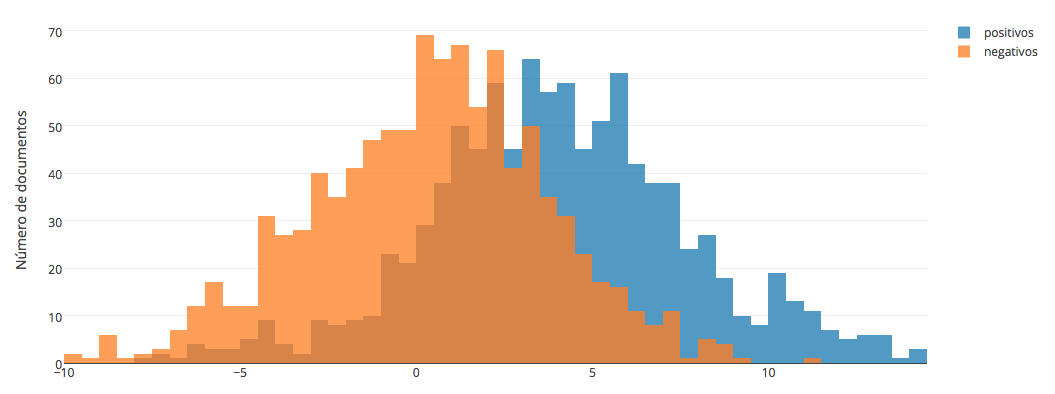
\includegraphics[scale=0.45]{movies_positive_to_negative_ratio_of_adjectives_sum_and_bigrams_with_adjectives}
\label{figura:movies_dist_1}
\end{figure}

\begin{figure}[H]
\caption{Distribuição dos valores da característica "A diferença entre as somas positiva e negativa de adjetivos e bigrams compostos estritamente por advérbio e adjetivo" na base de filmes}
\centering
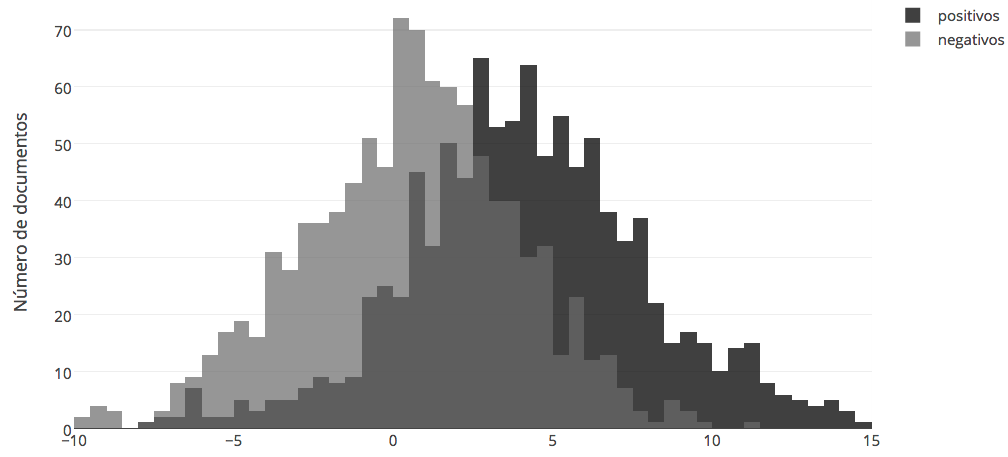
\includegraphics[scale=0.45]{movies_positive_to_negative_ratio_of_unigrams_and_bigrams_sum}
\label{figura:movies_dist_2}
\end{figure}


\begin{figure}[H]
\caption{Distribuição dos valores da característica "A diferença entre as somas positiva e negativa de adjetivos e bigrams compostos estritamente por advérbio e adjetivo" na base da Amazon}
\centering
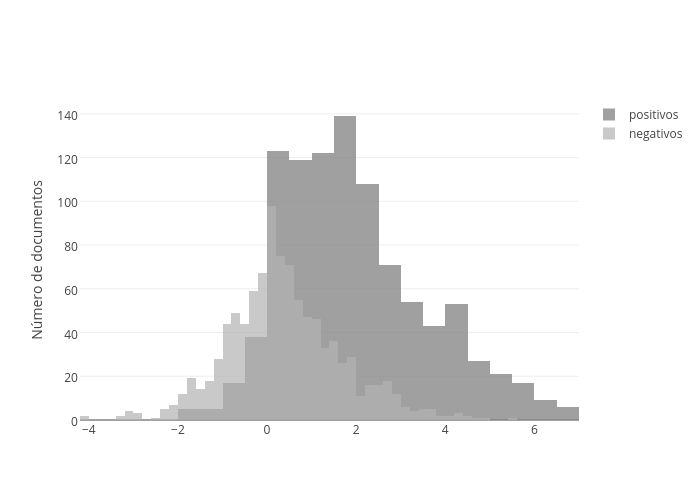
\includegraphics[scale=0.45]{amazon_positive_to_negative_ratio_of_adjectives_sum_and_bigrams_with_adjectives}
\label{figura:amazon_dist_1}
\end{figure}

\begin{figure}[H]
\caption{Distribuição dos valores da característica "A diferença entre as somas positiva e negativa de adjetivos e bigrams compostos estritamente por advérbio e adjetivo" na base da Amazon}
\centering
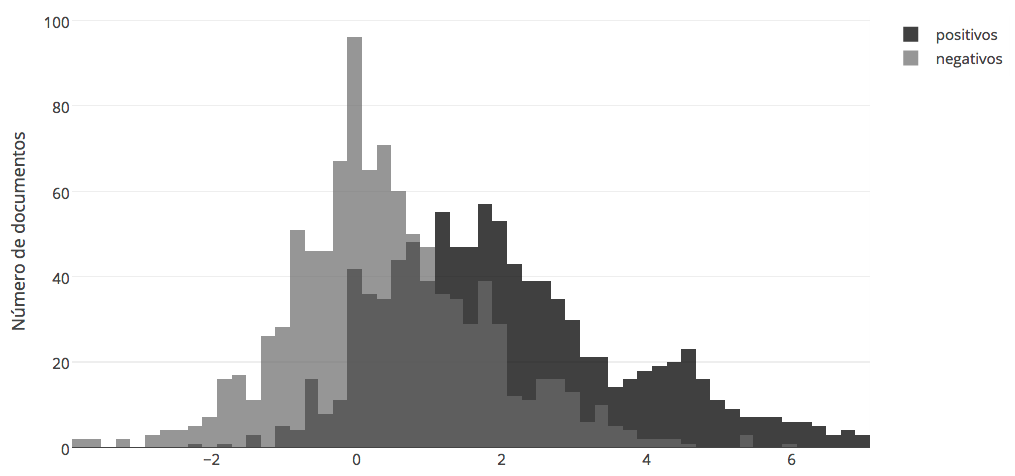
\includegraphics[scale=0.45]{amazon_positive_to_negative_ratio_of_unigrams_and_bigrams_sum}
\label{figura:amazon_dist_2}
\end{figure}

Na base de filmes, as características se aproximam de uma distribuição normal simétrica, enquanto na base da Amazon são mais assimétricas. Essa falta de equilibrio explica a mais significativa discrepância entre os valores de TPR  e TNR para o c4.5 na base da Amazon, enquanto que na base de filmes, o desequilíbrio entre essas duas medidas é menor. Lembrando mais uma vez que o CFS sofre menos com essa variação, pois há outras características para cobrir mais dados da base de testes.

\todo[inline]{a acurácia está péssima, quase jogar uma moeda, porque?}
\todo[inline]{o desvio padrão aqui chamada muita atenção, está muito muito alto, , mas o cfs tem desvio menos de TNR e TPR, mas o c4.5 consegui menor desvio de acurácia, porque?}
\todo[inline]{as caracteristicas selecionadas são sempre as mesmas? quantas diferentes? quais as mais populares? o CFS e c4.5 escolhem alguma caracteristica em comum? coloca no texto}
\todo[inline]{pega cada tabela para discutir o que ela apresenta, TNR, TPR, acurácia, caracteristicas selecionadas, não somente descreva mas tente discutir o que ocorreu, e complemente com informações que ajudam o leitor a saber o que está ocorrendo, como informando algo sobre as caracteristicas selecionadas, as regras geradas, etc}

%SVM Filmes

%---> Avg TPR:  69.1 %
%Standard Deviation:  7.3 %
%---> Avg TNR:  72.1 %
%Standard Deviation:  6.87677249878 %
%---> Avg acuracia:  70.6 %
%Standard Deviation:  3.44818792991 %

%WILCOXON
%two-tailed

%Result 1 - Z-value
%The Z-value is -1.1212. The p-value is 0.26272. The result is not significant at p≤ 0.01.
%
%Result 2 - W-value
%The W-value is 16.5. The critical value of W for N = 10 at p≤ 0.01 is 3. Therefore, the result is not significant at p≤ 0.01.


%SVM
%
%---> Avg TPR:  65.8 %
%Standard Deviation:  4.6432747065 %
%---> Avg TNR:  75.5 %
%Standard Deviation:  3.20156211872 %
%---> Avg acuracia:  70.65 %
%Standard Deviation:  2.99207286008 %

%WILCOSOX
%
%Result 1 - Z-value
%The Z-value is -2.3953. The p-value is 0.0164. The result is not significant at p≤ 0.01.
%
%Result 2 - W-value
%The W-value is 4. The critical value of W for N = 10 at p≤ 0.01 is 3. Therefore, the result is not significant at p≤ 0.01.

%Em ambas as bases as diferenças entre os resultados não são significativas usando o teste \textit{Wilcoxon signed-rank} para $p <= 0.01$. \todo[inline]{o teste foi para acurácia? tem que dizer qual medida foi utilizada} Isso mostra que mesmo que o CFS utiliza quase 5 vezes mais características em ambas as bases e não consegue produzir resultados significativamente melhores, criando ainda regras mais complexas e de difícil compreensão para seres humanos. Assim, já que o algoritmo c4.5 somente precisou de 2 características, produzindo regras menos complexas e mais claras, para produzir resultados próximos ou iguais ao do CFS, decidiu-se em manter o c4.5 para os próximos cenários de avaliação. 
\todo[inline]{c4.5 precisou de 2 caract? sua tabela indica 1 caracteristica, então seriam caracteristicas diferentes para cada base? ou na mesma base, folds diferentes? apresenta o histograma destas 2 caracteristicas para ilustar}

\todo[inline]{vocÊ consegue justificar porque o classificador estava jogando quase tudo para uma classe? o problema é na features selecionada, na modelagem do conjunto fuzzy, no metodo de inferencia? explica um pouco}

\todo[inline]{ressalte que os folds foram definidos por amostragem estratificada, mantendo a mesma proporção de documentos positivos e negativos do dataset total, e assim cada fold também está balanceado, isso ajuda a mostrar que um eventual enviesamento dos folds não foi a causa deste comportamento}

%\subsubsection{Avaliação do impacto da altura da árvore de decisão do algoritmo de seleção de características do c4.5}
\todo[inline]{acho melhor não fazer uma seção separada para arvore de altura  3, sugiro incorporar a seção anterior e incluir mais uma coluna nas tabelas, ficando c4.5 altura 1 e c4.5 altura 3}

%É importante ressaltar que os resultados anteriores, para o c4.5, foram obtidos com o algoritmo otimizado, utilizando a ferramenta Weka [CITE], para que a árvore do algoritmo de seleção de características do algoritmo tivesse altura 1, para fins de simplificação das regras geradas. Dessa forma, decidimos avaliar o quanto o aumento da altura da árvore de decisão do algoritmo de seleção de características do c4.5 influenciaria na classificação dos documentos. Definimos que o limite da altura da árvore de decisão fosse 3 para não aumentar demais a complexidade das regras que seriam geradas. A tabela (\ref{table:movies_h3}) e tabela (\ref{table:amazon_h3}) mostram, respectivamente, os resultados para este cenário nas bases de filmes e da Amazon.

\todo[inline]{o que seria 'algoritmo otimizado'? não devemos 'forçar' a arvore a ficar com altura 3, devemos dizer que utilizamos as características  selecionadas foram aquelas existentes até altura 3, porque se a árvore crescer além disso, é só ignorar os demais nós}

% \begin{table}[!h]
%    \begin{tabular}{lll}
%    Movies                                            & c4.5 - Altura 3                                          & c4.5 - Altura 1                               \\ \hline
%    TNR                                               & 55.6\% $\pm$ 43.49\%                            & 47.1\% $\pm$ 42.67\% \\
%    TPR                                               & 53.4\% $\pm$ 44.50\%                            & 61.7\% $\pm$ 43.93\% \\
%    acuracia                                      & 54.5\% $\pm$ 1.76\%                             & 54.4\% $\pm$ 1.72\% \\
%    Características selecionadas      & 1.1 $\pm$ 0.3                                           & 1                                     \\
%    \end{tabular}
%    \caption{Resultados da base de filmes}
%    \label{table:movies_h3}
%\end{table}

%Result 1 - Z-value
%
%The Z-value is -1.7838. The p-value is 0.07508. The result is not significant at p≤ 0.01.
%
%Result 2 - W-value
%
%The W-value is 10. The critical value of W for N = 10 at p≤ 0.01 is 3. Therefore, the result is not significant at p≤ 0.01.

%\begin{table}[!h]
%    \begin{tabular}{lll}
%    Movies                                              & c4.5 - Altura 3                               & c4.5 - Altura 1                              \\ \hline
%    TNR                                                     & 73.7\% $\pm$ 35.86\%                  & 34.0\% $\pm$ 43.26\%  \\
%    TPR                                                 & 47.1\% $\pm$ 34.22\%                  & 74.5\% $\pm$ 38.82\% \\
%    acuracia                                        & 60.4\% $\pm$ 5.75\%                       & 54.25\% $\pm$ 2.82\% \\
%    Características selecionadas        & 1.9 $\pm$ 0.7                                 & 1 $\pm$                                  \\
%    \end{tabular}
%    \caption{Resultados da base da Amazon}
%    \label{table:amazon_h3}
%\end{table}

\todo[inline]{nas tabelas que mostram resultado do c4.5 altura 3, indicam um valor baixo da quant media de caract selecionadas, a mesma caracteristica está sendo selecionada por vários nós? diga quais são e discuta no texto esse comportamento, isso pode indicar que uma característica é repeditamente relevante em vários splits dos dados (cada nó da árvore de decisão, divide a base para os nós seguintes)}

%Result 1 - Z-value
%
%The Z-value is -2.1915. The p-value is 0.02852. The result is not significant at p≤ 0.01.
%
%Result 2 - W-value
%
%The W-value is 6. The critical value of W for N = 10 at p≤ 0.01 is 3. Therefore, the result is not significant at p≤ 0.01.

%Mais uma vez, os resultados apresentados em ambas as bases para o aumento da altura da árvore de decisão do algoritmo de seleção de características não produziram resultados significativamente melhores para $p <= 0.01$ no teste \textit{Wilcoxon signed-rank}. \todo[inline]{sempre precisa dizer qual medida está sendo avalida pelo testes estatístico, reveja aqui e no restante do texto} Assim, o crescimento da árvore, que resulta no aumento da complexidade das regras em relação a altura 1, não contribui para o aumento de performance do nosso classificador e na simplificação das regras geradas para a classificação. 

\subsection{Avaliação dos sistemas de inferência fuzzy}

Nessa subseção são avaliados os desempenhos dos sistemas de inferência escolhidos, o Método do Raciocínio Fuzzy Geral (MRFG) e o Método do Raciocínio Fuzzy Clássico (MRFC). Os resultados mostram que em todos os cenários, independente do algoritmo de seleção usado, o MRFG produz melhores melhores percentuais de acurácia que o MRFC, mesmo que em alguns casos a diferença não seja significativa (para $p <= 0.01$). Isso indica que a abordagem do MRFC de analisar individualmente a classificação de um único documento em vez de analisar todo o conjunto de dados frente às regras, como faz o MRFG, é uma abordagem que tente a ter menos eficácia. É importante observar, contudo, que ambos os métodos apresentam altos desvios padrão nas medidas de TPR e TNR em todos os métodos de seleção, mostrando ainda instabilidade no sistema, como exemplificado na tabela \ref{table:movie_folds}, mesmo que menor. 

O uso de pesos nas regras, por outro lado, diminuiu bastante os desvios padrão de TPR e TNR, além de aumentar o desempenho geral (acurácia) do classificador em todos os cenários. Destaque principalmente para os cenários que usam o c.4.5, com menos características e, por conseguinte, menos regras, para a aumento significativo (para $p <= 0.01$) na base de filmes, usando c4.5 com altura 1 e o MRFG usando pesos, que saltou de 59,2\% (sem pesos) para 70,05\% de acurácia; e na base da Amazon, no mesmo cenário, saltando de 60,05\% para 70,85\% de acurácia. Ainda nesses cenários, os desvios padrão de TPR e TNR estavam acima de 30\% e, utilizando os pesos, caíram para menos de 10\% em filmes e 6\% na base mista da Amazon.

Isso acontece pois a aplicação dos pesos aumenta o espaço de cobertura das regras mais relevantes (ou com capacidade maior de classificar mais e melhor documentos) e diminui o espaço de regras que não tem a mesma importância e que são capazes de classificar somente uma menor região do espaço de dados. Por exemplo, as regras a seguir foram geradas um alguns dos folds para classificação usando c4.5 na base de filmes:

\begin{itemize}
\item Fold 0
\begin{itemize}
\item SE a diferença entre as somas positiva e negativa de adjetivos e bigrams compostos estritamente por advérbio e adjetivo é BAIXA então a polaridade é NEGATIVA;
\item SE a diferença entre as somas positiva e negativa de adjetivos e bigrams compostos estritamente por advérbio e adjetivo é MÉDIA então a polaridade é POSITIVA;
\item SE a diferença entre as somas positiva e negativa de adjetivos e bigrams compostos estritamente por advérbio e adjetivo é ALTA então a polaridade é POSITIVA;
\end{itemize}
\item Fold 1
\begin{itemize}
\item SE a diferença entre as somas positiva e negativa de unigrams e bigrams combinados é BAIXA então a polaridade NEGATIVA;
\item SE a diferença entre as somas positiva e negativa de unigrams e bigrams combinados é MÉDIA então a polaridade NEGATIVA;
\item SE a diferença entre as somas positiva e negativa de unigrams e bigrams combinados é ALTA então a polaridade POSITIVA;
\end{itemize}
\end{itemize}

Lembrando que "BAIXA", "MÉDIA" e "ALTA" são as modelagens dos conjuntos fuzzy para nossas variáveis de entrada e em quase todos os folds, as regras foram iguais. Contudo, em cada fold, as regras tem igual importância, quando não se utiliza os pesos. O resultado da classificação usando essas (e as demais geradas) com MRFG como sistema de inferência e sem pesos é apresentado na tabela \ref{table:movie_folds_2}.

\begin{table}[H]
	\centering
    \begin{tabular}{ll}
    Fold 0 \\ \hline
    Accuracy &  59.0\% \\
	TPR &  97.0\% \\
	TNR &  21.0\% \\ \\
	
	Fold 1 \\ \hline
    Accuracy &  57.5\% \\
	TPR &  17.0\% \\
	TNR &  98.0\% \\ \\
	
	Fold 2 \\ \hline
    Accuracy &  60.0\% \\
	TPR &  91.0\% \\
	TNR &  29.0\% \\ \\
	
	Fold 3 \\ \hline
    Accuracy &  60.0\% \\
	TPR &  98.0\% \\
	TNR &  22.0\% \\ \\
	
	Fold 4 \\ \hline
    Accuracy &  61\% \\
	TPR &  98.0\% \\
	TNR &  24.0\% \\ \\
	
	Fold 5 \\ \hline
    Accuracy &  55\% \\
	TPR & 14.0\% \\
	TNR &  99.0\% \\ \\
	
	Fold 6 \\ \hline
    Accuracy &  58\% \\
	TPR &  18.0\% \\
	TNR &  98.0\% \\ \\
	
	Fold 7 \\ \hline
    Accuracy &  60.5\% \\
	TPR &  94.0\% \\
	TNR &  27.0\% \\ \\
	
	Fold 8 \\ \hline
    Accuracy &  61.5\% \\
	TPR &  29.0\% \\
	TNR &  94.0\% \\ \\
	
	Fold 9 \\ \hline
    Accuracy &  59.5\% \\
	TPR &  90.0\% \\
	TNR &  29.0\% \\
    \end{tabular}
    \caption{Resultados com c4.5 e MRFG sem pesos - base de filmes}
    \label{table:movie_folds_2}
\end{table}

É possível perceber a instabilidade do sistema e recordar a tabela \ref{table:movies_3f} que nos mostra o resultado final de 59.2\% de acurácia, 53.8\% +- 34.96\% de TNR e 64.6\% +- 37.08\% com altos percentuais nos desvios padrão. O uso dos pesos, porém, vai alterar a importância entre as regras, enaltecendo àquelas mais aptas à classificação. As mesmas regras acima recebem os seguintes pesos:

\begin{itemize}
\item Fold 0
\begin{itemize}
\item SE a diferença entre as somas positiva e negativa de adjetivos e bigrams compostos estritamente por advérbio e adjetivo é BAIXA então a polaridade é NEGATIVA - \textbf{Grau: 0.60801671};
\item SE a diferença entre as somas positiva e negativa de adjetivos e bigrams compostos estritamente por advérbio e adjetivo é MÉDIA então a polaridade é POSITIVA - \textbf{Grau: 0.01536631};
\item SE a diferença entre as somas positiva e negativa de adjetivos e bigrams compostos estritamente por advérbio e adjetivo é ALTA então a polaridade é POSITIVA  - \textbf{Grau: 0.6912395};
\end{itemize}
\item Fold 1
\begin{itemize}
\item SE a diferença entre as somas positiva e negativa de unigrams e bigrams combinados é BAIXA então a polaridade NEGATIVA  - \textbf{Grau: 0.49867233};
\item SE a diferença entre as somas positiva e negativa de unigrams e bigrams combinados é MÉDIA então a polaridade NEGATIVA  - \textbf{Grau: 0.01143232};
\item SE a diferença entre as somas positiva e negativa de unigrams e bigrams combinados é ALTA então a polaridade POSITIVA  - \textbf{Grau: 0.67380056};
\end{itemize}
\end{itemize}

É possível perceber que as regras do conjunto "MEDIA" recebem os menores graus, enquanto que as regras dos conjuntos "BAIXA" e "ALTA" recebem os maiores - esse comportamento se repete para todos os demais folds. Isso mostra que o conjunto "BAIXA" e as regras relacionadas não são boas ou tão importantes para classificar os documentos usando essas características. Assim, a disputa entre as regras no momento da classificação ficará somente entre as demais. A tabela TAL mostra os resultados para a mesma configuração da tabela \ref{table:movie_folds_2}, excetuando o uso dos pesos. 

\begin{table}[H]
	\centering
    \begin{tabular}{ll}
    Fold 0 \\ \hline
    Accuracy &  71.0\% \\
	TPR &  65.0\% \\
	TNR &  77.0\% \\ \\
	
	Fold 1 \\ \hline
    Accuracy &  71.0\% \\
	TPR &  65.0\% \\
	TNR &  77.0\% \\ \
	
	Fold 2 \\ \hline
    Accuracy &  73.5\% \\
	TPR &  70.0\% \\
	TNR &  77.0\% \\ \
	
	Fold 3 \\ \hline
    Accuracy &  67.0\% \\
	TPR &  80.0\% \\
	TNR &  54.0\% \\ \\
	
	Fold 4 \\ \hline
    Accuracy &  75.5\% \\
	TPR &  80.0\% \\
	TNR &  71.0\% \\ \\
	
	Fold 5 \\ \hline
    Accuracy &  61.5\% \\
	TPR & 50.0\% \\
	TNR &  73.0\% \\ \\
	
	Fold 6 \\ \hline
    Accuracy &  67\% \\
	TPR &  58.0\% \\
	TNR &  76.0\% \\ \\
	
	Fold 7 \\ \hline
    Accuracy &  75\% \\
	TPR &  81.0\% \\
	TNR &  69.0\% \\ \\
	
	Fold 8 \\ \hline
    Accuracy &  69\% \\
	TPR &  71.0\% \\
	TNR &  67.0\% \\ \\
	
	Fold 9 \\ \hline
    Accuracy &  70\% \\
	TPR &  77.0\% \\
	TNR &  63.0\% \\
    \end{tabular}
    \caption{Resultados com c4.5 e MRFG sem pesos - base de filmes}
    \label{table:movie_folds_3}
\end{table}

Agora, diferentemente de antes, é possível perceber a maior estabilidade do sistema e recordar a tabela \ref{table:movies_3f} que nos mostra o resultado final de 70.05\% de acurácia, 70.4\% +- 7.11\% de TNR e 69.7\% +- 9.81\% com baixos percentuais nos desvios padrão.

%Da mesma maneira que foi feita na seção anterior, nós fixamos os demais parâmetros do experimento para melhor avaliar os sistemas de inferência, mantendo o algoritmo de seleção de característica c4.5 (com altura 1, para continuar buscando a geração de regras claras e de fácil leitura para humanos) e 3 conjuntos fuzzy nas variáveis de entrada. A tabela (\ref{table:movies2}) e tabela (\ref{table:amazon2}) mostram, respectivamente, os resultados para este cenário nas bases de filmes e da Amazon.
%
%\begin{table}[!h]
%    \begin{tabular}{lll}
%    ~                   & CFRM                              & GFRM \\ \hline
%    TNR                 & 47.1\% $\pm$ 42.67\%   & 53.8\% $\pm$ 34.96\%    \\
%    TPR             & 61.7\% $\pm$ 43.93\%   & 64.6\% $\pm$ 37.08\%   \\
%    acuracia        & 54.4\% $\pm$ 1.72\%       & 59.2\% $\pm$ 1.83\%    \\
%    \end{tabular}
%    \caption{Resultados dos sistemas de inferência na base de filmes}
%    \label{table:movies2}
%\end{table}

%Result 1 - Z-value
%
%The Z-value is -2.8031. The p-value is 0.00512. The result is significant at p≤ 0.01.
%
%Result 2 - W-value
%
%The W-value is 0. The critical value of W for N = 10 at p≤ 0.01 is 3. Therefore, the result is significant at p≤ 0.01.

%\begin{table}[!h]
%    \begin{tabular}{lll}
%    ~                   & CFRM                                  & GFRM \\ \hline
%    TNR                 & 34.0\% $\pm$ 43.26\%      & 44.6\% $\pm$ 35.73\%    \\
%    TPR             & 74.5\% $\pm$ 38.82\%      & 75.5\% $\pm$ 34.80\%    \\
%    acuracia        & 54.25\% $\pm$ 2.82\%      & 60.05\% $\pm$ 2.37\%   \\
%    \end{tabular}
%    \caption{Resultados dos sistemas de inferência na base da Amazon}
%    \label{table:amazon2}
%\end{table}

%Result 1 - Z-value
%
%The Z-value is -2.8031. The p-value is 0.00512. The result is significant at p≤ 0.01.
%
%Result 2 - W-value
%
%The W-value is 0. The critical value of W for N = 10 at p≤ 0.01 is 3. Therefore, the result is significant at p≤ 0.01.

%Os resultados mostram que Método Geral do Raciocínio Fuzzy (MRFG) aumenta o \textit{acuracia} sobre o MRFC, em ambas bases,  mantendo a seleção de características e a quantidade de conjuntos fuzzy inalterados. O resultado do teste \textit{Wilcoxon signed-rank} confirma a melhora significativa do MRFG sobre o MRFC, para $p <= 0.01$. Assim, nessa tarefa de classificação de somente duas classes, positivo e negativo, os resultados mostraram que uma melhor abordagem é considerar todas as regras de uma classe, em vez de uma única com maior grau. Daí, o MRFG foi a nossa escolha para prosseguir nos próximos experimentos com o fim de alcançar melhores resultados nesse trabalho.

%\subsection{Avaliação de uso de pesos nas regras dos sistemas de inferência}
%
%Em \cite{ishibuchi2001effect} foi mostrado que é possível aumentar a performance da classificação de regras fuzzy IF-THEN, aplicando pesos à elas, além do grau de compatibilidade das regras. No referido artigo, os autores descreveram o processo em que é possível melhorar o desempenho da classificação sem alterar os conjuntos fuzzy das variáveis de saída e de entrada. Baseando-se neste artigo, este trabalho calculou os pesos como se segue. Para cada regra da base de regras gerada, foi calculado o grau de compatibilidade com todos documentos do conjunto de teste. Se o documento fosse positivo, o grau de compatibilidade era acumulado em $\beta_{positivo}$; se o documento fosse negativo, o grau de compatibilidade era acumulado em $\beta_{negativo}$. Ao fim desse processo, caso ambos os betas fosse iguais, não haveria peso a ser considerado, já que as regras tem igual influência sobre o conjunto de dados que elas foram geradas. De outra forma, o peso da regra era definido pela equação \ref{eq:pesos}.
%
%\begin{equation}
%P_j = |\beta_{positivo} - \beta_{negativo}| / (\beta_{positivo} + \beta_{negativo})
%\label{eq:pesos}
%\end{equation}
%
%onde $P_j$ é o peso da regra, para $0 <= P_j <= 1$. 

\todo[inline]{discuta qual é idéia por trás do uso de pesos, valorizar regras que de fato auxiliar a distinguir as duas classes e desvalorizar aquelas que não conseguem separar as classes}

%Uma vez que todas as regras tiveram seus pesos calculados, estes são adicionados ao processo de classificação de ambos os métodos utilizados até aqui, o MRFG e o MRFC. O peso torna-se um fator multiplicador do grau de cada regra. Assim, o MRFC em vez de somente levar em consideração a regra com maior grau de compatibilidade com o documento de teste, vai, agora, levar em consideração a regra com maior grau multiplicado pelo peso da regra. O mesmo acontece para o MRFG ao considerar o grau médio entre as classes positivo e negativo. A tabela (\ref{table:movies2_pesos}) e tabela (\ref{table:amazon2_pesos}) mostram, respectivamente, os resultados para o uso dos pesos nas bases de filmes e da Amazon usando os parâmetros até agora estabelecidos. 

\todo[inline]{discuta mais esses resultados, há uma grande mudança qualitativa dos resultados com uso de pesos, principalmente porque o desvio padrão cai muito, quais foram as regras que ganharam pesos e quais perderam peso? quais os valores de pesos encontrados, são próximos dos valores extremos, 0 e 1? como isso ajuda a explicar os resultados ruins sem peso? discuta o desvio padrão também }

%\todo[inline]{as tabelas são para classico ou geral?}
%\begin{table}[!h]
%    \begin{tabular}{lll}
%    ~                   & S/ Pesos                              & C/ Pesos \\ \hline
%    TNR                 & 53.8\% $\pm$ 34.96\%      & 70.4\% $\pm$ 7.11\%    \\
%    TPR             & 64.6\% $\pm$ 37.08\%      & 69.7\% $\pm$ 9.81\%   \\   
%    acuracia        & 59.2\% $\pm$ 1.83\%       & 70.05\% $\pm$ 4.00\%    \\
%    \end{tabular}
%    \caption{Resultados dos sistemas de inferência na base de filmes utilizando pesos nas regras}
%    \label{table:movies2_pesos}
%\end{table}

%Result 1 - Z-value
%
%The Z-value is -2.8031. The p-value is 0.00512. The result is significant at p≤ 0.05.
%
%Result 2 - W-value
%
%The W-value is 0. The critical value of W for N = 10 at p≤ 0.05 is 8. Therefore, the result is significant at p≤ 0.05.

%\begin{table}[!h]
%    \begin{tabular}{lll}
%    ~                   & S/ Pesos                                  & C / Pesos \\ \hline
%    TNR                 & 44.6\% $\pm$ 35.73\%      & 76.80\% $\pm$ 4.57\%    \\
%    TPR             & 75.5\% $\pm$ 34.80\%      & 64.9\% $\pm$ 5.50\%    \\
%    acuracia        & 60.05\% $\pm$ 2.37\%      & 70.85\% $\pm$ 3.09\%   \\
%    \end{tabular}
%    \caption{Resultados dos sistemas de inferência na base da Amazon utilizando pesos nas regras}
%    \label{table:amazon2_pesos}
%\end{table}

%Result 1 - Z-value
%
%The Z-value is -2.8031. The p-value is 0.00512. The result is significant at p≤ 0.05.
%
%Result 2 - W-value
%
%The W-value is 0. The critical value of W for N = 10 at p≤ 0.05 is 8. Therefore, the result is significant at p≤ 0.05.

%Os resultados corroboraram as conclusões de \cite{ishibuchi2001effect} que é possível melhorar o desempenho da classificação sem alterar os conjuntos fuzzy das variáveis de saída e de entrada apenas aplicando pesos às regras geradas. O resultado do teste \textit{Wilcoxon signed-rank} também confirma a melhora significativa do MRFG usando pesos nas regras em vez de somente o grau de compatibilidade, para $p <= 0.01$.

\section{Avaliação com o uso de 2 conjuntos fuzzy}
\subsection{Avaliação dos algoritmos de seleção de características}
\subsection{Avaliação dos sistemas de inferência fuzzy}


\todo[inline]{AINDA A REFAZER.}

%Através das últimas seções, foram mostrados resultados utilizando 3 conjuntos fuzzy para modelar nossas variáveis lingüísticas. Seguindo a nossa decisão de usar o c4.5 com altura máxima da árvore de decisão para 1 para reduzir a complexidade das regras geradas e torna-las mais legíveis para seres humanos, nós tentamos reduzir a quantidade de conjuntos fuzzy, usando somente os conjuntos "Baixo" e "Alto", para as variáveis de entrada. Esse experimento tem por fim verificar se há aumento da performance da classificação com regras mais simples e gerais. A tabela (\ref{table:movies2_pesos_2f}) e tabela (\ref{table:amazon2_pesos_2fs}) mostram, respectivamente, os resultados para o uso de somente dois conjuntos fuzzy nas variáveis de entrada nas bases de filmes e da Amazon.
%
%\begin{table}[!h]
%    \begin{tabular}{lll}
%    ~                   & 3 conjuntos fuzzy                             & 2 conjuntos fuzzy \\ \hline
%    TNR                 & 70.4\% $\pm$ 7.11\%                   & 71.2\% $\pm$ 4.33\%    \\
%    TPR             & 69.7\% $\pm$ 9.81\%                   & 70.6\% $\pm$ 3.35\%   \\
%    acuracia        & 70.05\% $\pm$ 4.00\%              & 70.9\% $\pm$ 3.07\%    \\
%    \end{tabular}
%    \caption{Resultados dos sistemas de inferência na base de filmes utilizando 2 conjuntos fuzzy na entrada}
%    \label{table:movies2_pesos_2fs}
%\end{table}
%
\todo[inline]{parece haver um redução no desvio padrão com uso de 2 conjuntos, porque será que reduziu?}
%
%%Result 1 - Z-value
%%
%%The Z-value is -1.2741. The p-value is 0.20408. The result is not significant at p≤ 0.05.
%%
%%Result 2 - W-value
%%
%%The W-value is 15. The critical value of W for N = 10 at p≤ 0.05 is 8. Therefore, the result is not significant at p≤ 0.05.
%
%\begin{table}[!h]
%    \begin{tabular}{lll}
%    ~                   & 3 conjuntos fuzzy                             & 2 conjuntos fuzzy \\ \hline
%    TNR                 & 76.80\% $\pm$ 4.57\%              & 77.2\% $\pm$ 3.54\%    \\
%    TPR             & 64.9\% $\pm$ 5.50\%                   & 64.4\% $\pm$ 3.46\%   \\
%    acuracia        & 70.85\% $\pm$ 3.09\%              & 70.8\% $\pm$ 3.27\%    \\
%    \end{tabular}
%    \caption{Resultados dos sistemas de inferência na base da Amazon utilizando 2 conjuntos fuzzy na entrada}
%    \label{table:amazon2_pesos_2fs}
%\end{table}
%
%%Result 1 - Z-value
%%
%%The Z-value is -0.3568. The p-value is 0.71884. The result is not significant at p≤ 0.01.
%%
%%Result 2 - W-value
%%
%%The W-value is 24. The critical value of W for N = 10 at p≤ 0.01 is 3. Therefore, the result is not significant at p≤ 0.01.
%
%A tabela (\ref{table:movies2_pesos_2fs}) mostra pequena melhora na base de filmes e empate técnico na base da Amazon. Mas, estatisticamente, os resultados não são significativamente diferentes para $p <= 1$. Todavia, a redução da quantidade dos conjuntos fuzzy para as variáveis de entrada produz regras mais simples e legíveis para serem humanos. Assim, nós temos regras menos complexas com a mesma performance de regras com maior número de antecedentes. 
%
%%positive_to_negative_ratio_of_adjectives_sum_and_bigrams_with_adjectives
%%positive_to_negative_ratio_of_unigrams_and_bigrams_sum
%Em ambos conjuntos de dados somente duas características foram selecionadas pelo c4.5:
%\begin{itemize}
%\item Diferença entre a soma positiva e negativa dos adjetivos e dos bigrams formados por advérbio e adjetivo
%\item Diferença entre a soma positiva e negativa dos unigrams e bigrams
%\end{itemize}
%
%Na base de filmes as duas foram necessárias para atingir os resultados mostrados na tabela ((\ref{table:movies2_pesos_2fs})). Isso remete ao fato de documentos de filmes serem mais difíceis de ser classificados, precisando de mais características para caracterizar corretamente as opiniões \cite{turney2002thumbs, pang2004sentimental, chaovalit2005movie, ohana2009sentiment}. Já na base da Amazon, somente a segunda característica foi utilizada para classificar os documentos. Embora o algoritmo de seleção de características do c4.5 tenha decidido que somente essa característica seja suficiente, não é difícil concluir que, sendo a base da Amazon bastante diversa (e que também inclui filmes), mais características podem ser necessárias para caracterizar melhor documentos tão variados.
%Todavia, nós conseguimos classificar um pouco mais de 70\% dos documentos de filmes e da Amazon com poucas regras simples, legíveis para humanos, geradas pelo método de Wang-Mendel:
%
%\begin{itemize}
%\item IF a \textit{diferença entre a soma positiva e negativa dos unigrams e bigrams} is ALTO then POLARIDADE is POSITIVA
%\item IF a \textit{diferença entre a soma positiva e negativa dos unigrams e bigrams} is BAIXO then POLARIDADE is NEGATIVA
%\item IF a \textit{diferença entre a soma positiva e negativa dos adjetivos e dos bigrams formados por advérbio e adjetivo} is ALTO then POLARIDADE is POSITIVA
%\item IF a \textit{diferença entre a soma positiva e negativa dos adjetivos e dos bigrams formados por advérbio e adjetivo} is BAIXO then POLARIDADE is NEGATIVA
%\end{itemize}
%
%As quatro regras foram utilizadas na base de filmes e as duas primeiras regras na base da Amazon.

\section{Avaliação do uso de regras entre domínios}
\todo[inline]{faz aplicação cruzada tambem, amazon na de filmes e vice versa}
\todo[inline]{valorize mais esta seção, o resultado é MUITO interessante, mas o texto não valoriza tanto, compare com os resultados de epinions com regras amazon e filmes. Quando aplicar amazon em filmes e vice versa compare com os resultados obtidos usando as regras da própria base. O uso do classificador de uma base em outra pode indicar a existencia de regras universais e realmente independentes de domínio, mas pode haver necessidade de ajuste na modelagem dos conjuntos ou em outro aspecto talvez}

Outra avaliação que fizemos foi a validação do uso de regras entre domínios, utilizando a base inteira da Epinions como teste. Foram usadas as regras geradas da base de filmes e da base da Amazon e aplicadas à base da Epinions. \todo[inline]{foram usadas as regras geradas para qual fold amazon ou filmes?} Para isso, a base da Epinions passou por pré-processamento, transformação e extração de características, para que as regras pudessem avaliar corretamente os documentos. É importante frisar que nenhuma adaptação foi feita às regras para que pudesse funcionar corretamente. Da maneira que foram geradas na bases de filmes e Amazon, foram utilizadas na classificação dos documentos da base da Epinions. A tabela \ref{table:epinions} mostra os resultados obtidos.
\todo[inline]{nenhuma mudança foi feita nas regras fuzzy, mas nenhuma foi feita também nas características selecionadas e na modelagem dos conjuntos, então reforça isso tambem}

\begin{table}[!h]
    \begin{tabular}{lll}
    ~               & Regras da Amazon                  & Regras dos Filmes \\ \hline
    TNR             & 47.05\% $\pm$ 0.35\%           & 61.7\% $\pm$ 1.41\%    \\
    TPR         & 90.5\% $\pm$ 1.11\%               & 85.8\% $\pm$ 1.22\%   \\
    acuracia    & 68.77\% $\pm$ .0.17\%             & 73.75\% $\pm$ 0.27\%    \\
    \end{tabular}
    \caption{Resultados da aplicação de regras da base de filmes e Amazon na base Epinions}
    \label{table:epinions}
\end{table}

Os resultados mostram que as regras geradas podem ser usadas entre domínios diferentes, produzindo resultados próximos ou melhores que os produzidos nas próprias bases, como pode ser visto na tabela \ref{table:epinions}.

\section{Outros resultados}

Cinquenta e sete características foram extraídas dos documentos para realizar os experimentos dessa pesquisa. Destas, duas foram constantemente selecionadas pelos algoritmos de seleção de características. Foram elas:
\todo[inline]{quantifica 'constantemente selecionadas', por exemplo em todas as configurações avaliadas elas sempre foram selecionadas? só com c4.5? }
\begin{itemize}
\item Diferença entre a soma positiva e negativa dos adjetivos e dos bigrams formados por advérbio e adjetivo
\item Diferença entre a soma positiva e negativa dos unigrams e bigrams
\end{itemize}

Essas características englobam unigrams e bigrams formados por advérbios e adjetivos. Esses resultados corroboram quase que completamente os n-grams propostos por \cite{turney2002thumbs}, formados em sua maioria por advérbios e adjetivos; reiteram também a importância central dos adjetivos na mineração e classificação de opiniões, como apontado por \cite{voll2007not}; além de reforçar o proposto por \cite{benamara2007sentiment} que advérbios tema significativa influência como modificadores de intensidade dos adjetivos.

Também comparamos a configuração final do nosso classificador com um método clássico de aprendizado de máquina muito utilizado na tarefa de mineração de opinião, o \textit{Support Vector Machine} (SVM), e que geralmente produz bons resultados, como ser visto em \cite{moraes2012document}, \cite{pang2002thumbs}, \cite{pang2004sentimental} e \cite{wilson2004just}. 

\begin{table}[!h]
    \begin{tabular}{lll}
    ~                   & Wang-Mendel 2 conjuntos fuzzy                     & SVM \\ \hline
    TNR                 & 71.2\% $\pm$ 4.33\%                                           & 72.9\% $\pm$ 5.80\%    \\
    TPR             & 70.6\% $\pm$ 3.35\%                                       & 68.6\% $\pm$ 7.04\%   \\
    acuracia        & 70.9\% $\pm$ 3.07\%                                       & 70.75\% $\pm$ 3.70\%    \\
    \end{tabular}
    \caption{Comparação entre os resultados do método de Wang-Mendel e SVM na base de filmes}
    \label{table:movies_svm}
\end{table}

%Result 1 - Z-value
%
%The Z-value is -0.5606. The p-value is 0.57548. The result is not significant at p≤ 0.01.
%
%Result 2 - W-value
%
%The W-value is 22. The critical value of W for N = 10 at p≤ 0.01 is 3. Therefore, the result is not significant at p≤ 0.01.

\begin{table}[!h]
    \begin{tabular}{lll}
    ~                       & Wang-Mendel 2 conjuntos fuzzy                             & SVM \\ \hline
    TNR                     & 77.2\% $\pm$ 3.54\%                                               & 75.5\% $\pm$ 3.20\%    \\
    TPR                 & 64.4\% $\pm$ 3.46\%                                               & 65.8\% $\pm$ 4.64\%   \\
    acuracia           & 70.8\% $\pm$ 3.27\%                                            & 70.65\% $\pm$ 2.99\%    \\
    \end{tabular}
    \caption{Comparação entre os resultados do método de Wang-Mendel e SVM na base da Amazon}
    \label{table:amazon_svm}
\end{table}

%Result 1 - Z-value
%
%The Z-value is -1.2232. The p-value is 0.22246. The result is not significant at p≤ 0.01.
%
%Result 2 - W-value
%
%The W-value is 15.5. The critical value of W for N = 10 at p≤ 0.01 is 3. Therefore, the result is not significant at p≤ 0.01.

Nossos resultados mostram que o classificador construído nesse trabalho equivale aos resultados do SVM, pois em ambas as bases as diferenças dos resultados não são significativas para $p <= 0.01$. Contudo, nosso classificador possui regras legíveis para seres humanos, é independente de domínio e não precisa de nova rodada de treino para diferentes bases, diferentemente do SVM.

\todo[inline]{falta uma seção final de discussão geral dos resultados para fechar esse capítulo, revisando os achados e fazendo uma avaliação geral de tudo}

\end{document}